\subsection{Tinte en CIELAB}
\label{sec:tinte}

El tinte (\archivo{coloring/dye.py}) recibe una máscara suave del pelo $\alpha\in[0,1]$ y un color objetivo con componentes $(L_t,a_t,b_t)$ en CIELAB. La figura~\ref{fig:diag-tinte} resume el proceso.

\begin{figure}[ht]
  \centering
  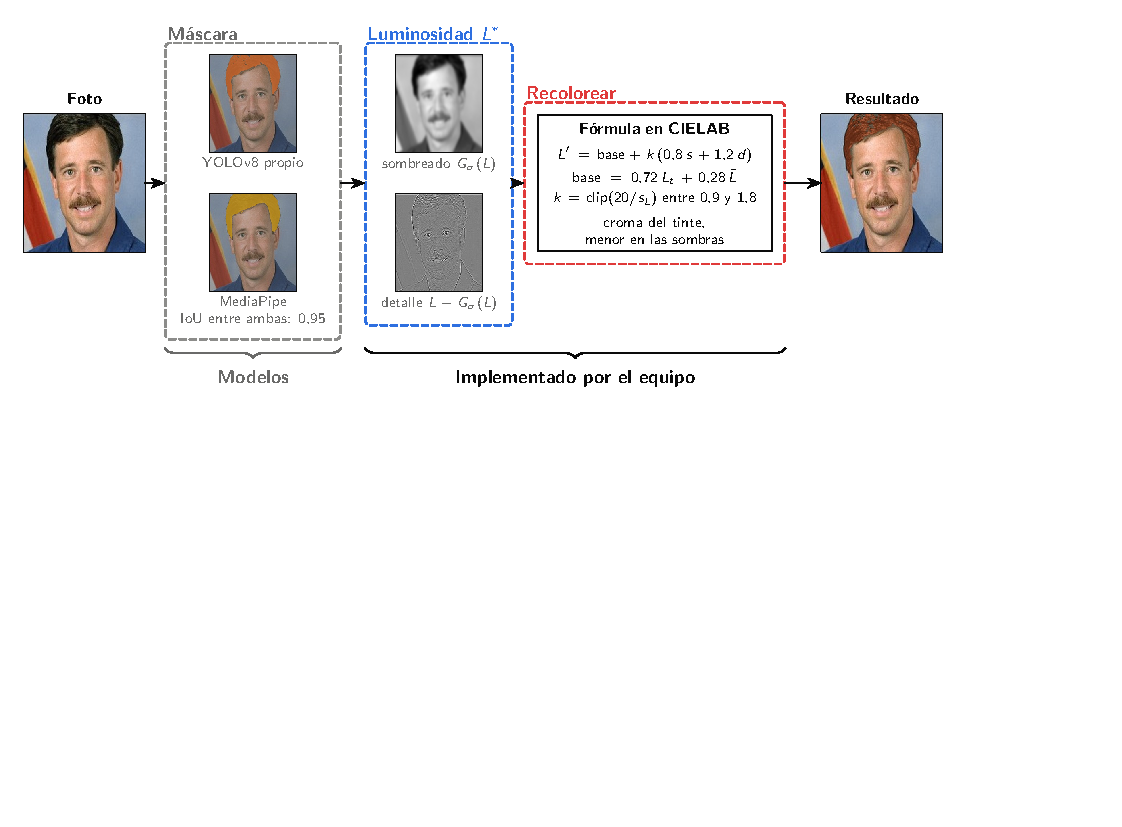
\includegraphics[width=\linewidth]{diagrama_tinte.pdf}
  \caption{Pipeline del tinte: máscara de YOLO o MediaPipe, separación de la luminosidad en sombreado y detalle, y recoloreo en CIELAB.}
  \label{fig:diag-tinte}
\end{figure}


\textbf{Por qué CIELAB.} En una primera versión se cambiaba el tono en HSV. Eso conserva la oscuridad del pelo, así que un pelo negro nunca podía quedar rubio. En CIELAB la luminosidad está separada del color, así que se puede mover la luminosidad base hacia la del tinte sin perder el detalle de cada mechón.

\textbf{Paso 1: luminosidad.} Sean $\bar L$ y $s_L$ la media y la desviación de $L^*$ dentro del pelo, y $G_\sigma$ un desenfoque gaussiano con $\sigma=1{,}5$~px. La imagen se descompone en sombreado (variación lenta) y detalle (mechones):
\begin{align}
  \text{detalle}&=L-G_\sigma(L), & \text{sombreado}&=G_\sigma(L)-\bar L,\\
  L' &= \underbrace{0{,}72\,L_t+0{,}28\,\bar L}_{\text{base}}+k\,(0{,}8\,\text{sombreado}+1{,}2\,\text{detalle}),
  & k&=\operatorname{clip}(20/s_L,\;0{,}9,\;1{,}8).
\end{align}
El factor $k$ normaliza el contraste: un pelo de contraste bajo, como uno negro liso, gana detalle, y uno muy contrastado no se exagera.

\textbf{Paso 2: color.} El croma se toma del tinte y se atenúa en las sombras más profundas, como ocurre con un pigmento real:
\begin{equation}
  a'=128+(a_t-128)\,(0{,}4+0{,}5\,d),\qquad d=\operatorname{clip}\!\left(\frac{L'}{\max(L_t,40)},0,1\right),
\end{equation}
y lo mismo para $b'$.

\textbf{Paso 3: mezcla.} El resultado se mezcla con la imagen original según $\alpha$ multiplicado por la intensidad elegida.

\textbf{Máscara.} La máscara viene de MediaPipe o del YOLO propio (sección~\ref{sec:segmentacion}). Su borde se suaviza hacia adentro, para no teñir la piel ni el fondo.

\subsection{Motor de cortes de pelo}
\label{sec:corte}

El corte es la pieza más compleja de la interfaz de estilos (\archivo{compositing/haircut.py}). Para cortar el pelo hay que resolver cuatro problemas:
\begin{enumerate}
  \item quitar el pelo que sobra y reconstruir lo que había detrás;
  \item saber dónde termina realmente la cabeza;
  \item ubicar la línea del pelo aunque haya flequillo;
  \item hacer crecer pelo corto creíble, con la luz de la foto.
\end{enumerate}
La figura~\ref{fig:diag-corte} muestra las etapas sobre un retrato.

\begin{figure}[ht]
  \centering
  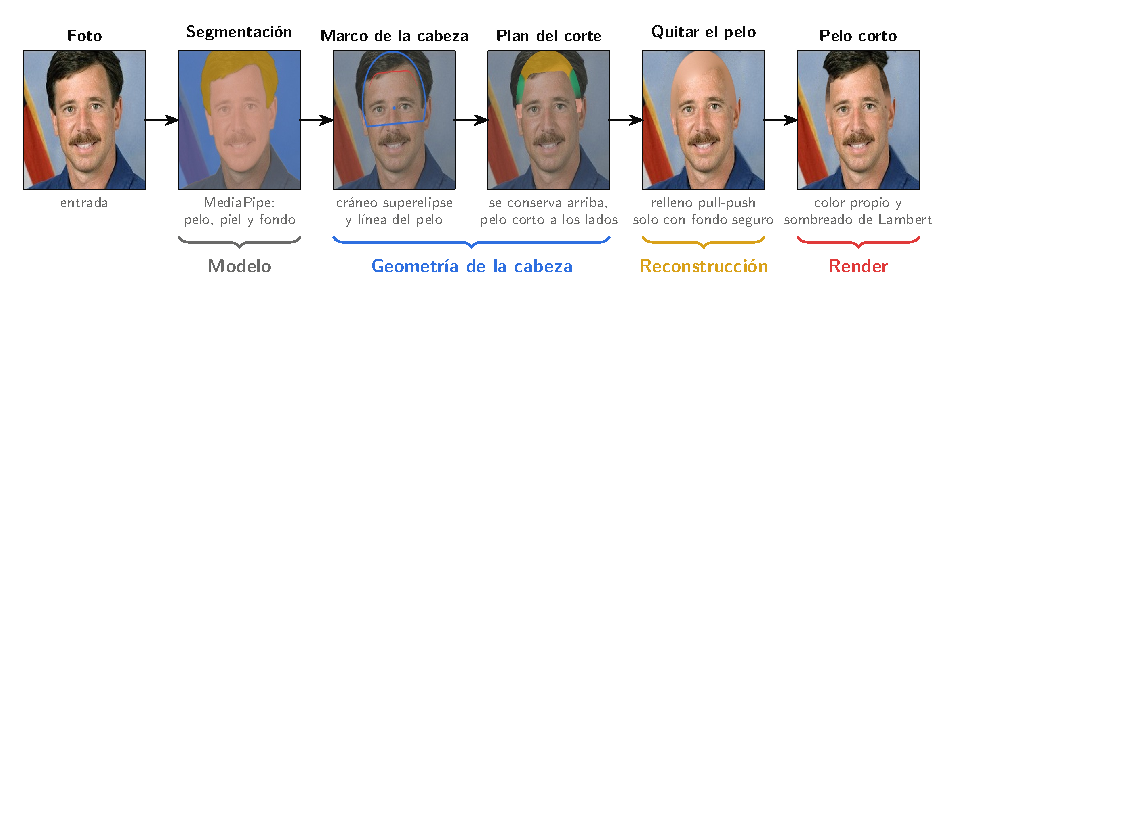
\includegraphics[width=\linewidth]{diagrama_corte.pdf}
  \caption{Pipeline del corte (degradado medio): segmentación, marco de la cabeza con el cráneo y la línea del pelo, plan del corte, relleno con \emph{pull-push} y pelo corto sombreado.}
  \label{fig:diag-corte}
\end{figure}

\textbf{Resolución de trabajo.} El corte se calcula sobre un recorte de la cabeza escalado para que el ancho de la cabeza mida 420~px. Al volver a la resolución original se suma de nuevo el detalle de alta frecuencia de la foto en las zonas que no cambiaron. Así una foto de 4000~px tarda lo mismo que una de 800~px y no pierde nitidez.

\textbf{Línea del pelo.} Primero se busca la frente visible: desde las cejas se sube por la columna central mientras la probabilidad de piel de la cara sea alta.
\begin{itemize}
  \item Si se ven al menos $0{,}2\,w$ de frente, el borde de esa piel es la línea del pelo real.
  \item Si no, hay flequillo, y se asume una frente típica de $0{,}30\,w$ sobre las cejas, en línea con las proporciones faciales de \cite{farkas1994}.
\end{itemize}
Hacia los costados, la línea se retrae un poco en las sienes y baja hasta la patilla con una esquina redondeada (un cuarto de circunferencia). Se le añade un ruido de baja frecuencia para que no sea una línea perfecta.

\textbf{Cráneo.} La cabeza rapada es una superelipse de exponente 2{,}15 en el marco $(x,y)$:
\begin{equation}
  \left|\frac{x}{0{,}55}\right|^{2{,}15}+\left|\frac{\min(y,0)}{y_{\text{tope}}}\right|^{2{,}15}\le1.
\end{equation}
Sus costados bajan hasta las orejas. La altura $y_{\text{tope}}$ se ajusta a cada persona: es la mayor entre la línea del pelo menos $0{,}33\,w$ y la coronilla medida (el punto más alto de pelo o piel en la columna central) más $0{,}03\,w$. Si el pelo ya es corto, el cráneo no sobresale de la silueta real. Por último, el cráneo se intersecta con la silueta de la persona, ligeramente dilatada.

\textbf{Relleno del fondo con \emph{pull-push}.} El pelo que queda fuera del cráneo hay que quitarlo. El primer intento usó \emph{inpainting} de Telea \cite{telea2004}, que propaga el color de todo el borde del hueco; como ese borde incluye pelo, arrastraba el pelo hacia el fondo y dejaba ``pelo fantasma''. La solución es \emph{pull-push} \cite{gortler1996} con una máscara de píxeles conocidos elegida a mano:
\begin{itemize}
  \item cuentan solo los píxeles de fondo seguro ($p_{\text{fondo}}>0{,}6$) o de ropa, fuera del pelo;
  \item cerca del pelo se exige $p_{\text{fondo}}>0{,}9$.
\end{itemize}
En cada nivel de la pirámide, el color es $\sum w\,c/\sum w$, y en la fase \emph{push} se mezcla con el nivel grueso según el peso, $\operatorname{clip}(2w,0,1)$. La figura~\ref{fig:pullpush} compara ambos métodos.

Después del relleno se buscan \textbf{mechones sueltos}: píxeles cerca del hueco que se diferencian del fondo suavizado en más de 30 niveles. Se agregan al hueco y se rellena de nuevo. Además, el fondo rellenado recibe un ruido cuya amplitud es la energía de alta frecuencia local del fondo, propagada también con \emph{pull-push}, para que no se vea más liso que el resto.

\begin{figure}[ht]
  \centering
  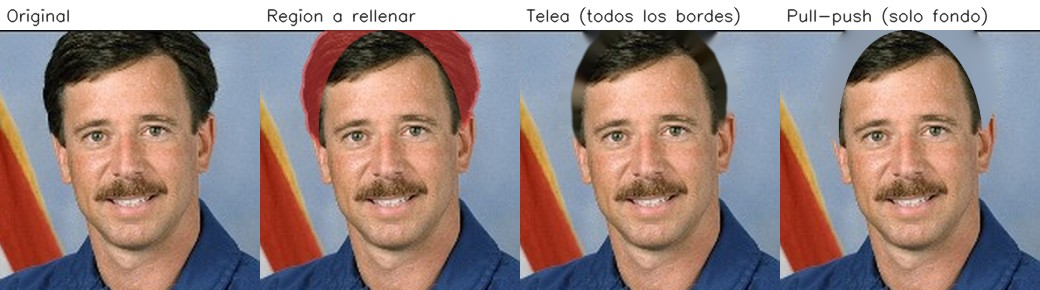
\includegraphics[width=\linewidth]{pull_push.jpg}
  \caption{Rellenar el fondo donde se quita pelo. Telea toma color de todo el borde y arrastra el pelo; \emph{pull-push} con solo píxeles de fondo deja un relleno limpio.}
  \label{fig:pullpush}
\end{figure}

\textbf{Piel bajo el pelo.} Dentro del cráneo, la piel que tapaba el pelo (cuero cabelludo o frente bajo un flequillo) se rellena con \emph{pull-push}. Como fuente se usan solo píxeles de piel de la cara alejados del pelo, porque la piel pegada a la línea del pelo suele estar sombreada y dejaba una marca. La transición hacia la piel real es gradual.

\textbf{Pelo corto.} El pelo nuevo tiene el color del propio pelo: la mediana en CIELAB del 45~\% más oscuro de los píxeles de pelo. Se sombrea con un modelo de Lambert \cite{marschner2016}:
\begin{itemize}
  \item la normal sale de tratar el cráneo como un elipsoide;
  \item la dirección de la luz se estima de la asimetría de brillo entre las dos mitades de la cara, más una componente desde arriba;
  \item la luminosidad final es $L=L_{\text{pelo}}\,(0{,}55+0{,}6\,s)$, donde $s=0{,}62+0{,}38\max(0,\hat n\cdot\hat l)$ es el sombreado.
\end{itemize}
La textura combina dos ruidos: uno anisótropo (desenfoque gaussiano mucho más largo en vertical que en horizontal) que imita trazos cortos, y uno de baja frecuencia para variaciones de densidad. La cobertura del pelo corto es
\begin{equation}
  c = \rho(x,y)\cdot z_{\text{pelo}}\cdot h_{\text{cráneo}}\cdot(1+0{,}08\,n_{\text{trazo}}+0{,}06\,n_{\text{parche}}),
\end{equation}
donde $z_{\text{pelo}}$ vale 1 por encima de la línea del pelo y $\rho$ es la densidad del estilo. La densidad base depende de la intensidad elegida $t$: $\rho_0=0{,}92\,(1{,}1-0{,}4\,t)$. Más intensidad significa pelo más corto, con más cuero cabelludo visible.

\textbf{Estilos.} Todos los cortes se definen sobre el mismo marco. La parte de arriba se conserva dentro de una franja $|x|<r(y)$, con
\begin{equation}
  r(y)=0{,}36+0{,}16\,\operatorname{smoothstep}\!\left(\frac{-0{,}40-y}{0{,}25}\right),
\end{equation}
que se ensancha hacia la coronilla. En los costados, la densidad sube desde la piel en $y_{\text{piel}}$ hasta pelo corto en $y_{\text{corto}}$:
\begin{equation}
  \rho(y)=\rho_0\,\min\!\Big(f+(1-f)\sqrt{\operatorname{smoothstep}\big(\tfrac{y_{\text{piel}}-y}{y_{\text{piel}}-y_{\text{corto}}}\big)},\;c_{\max}\Big),
\end{equation}
donde $f$ es la densidad mínima y $c_{\max}$, la máxima. La tabla~\ref{tab:cortes} da los parámetros.

\begin{table}[ht]
\centering
\small
\begin{tabularx}{\linewidth}{@{}l c c X@{}}
\toprule
Corte & $y_{\text{piel}}$ & $y_{\text{corto}}$ & Particularidad \\
\midrule
Degradado bajo & 0{,}10 & $-0{,}12$ & Piel solo junto a la oreja. \\
Degradado medio & $-0{,}08$ & $-0{,}30$ & Piel hasta la sien. \\
Degradado alto & $-0{,}24$ & $-0{,}46$ & Piel hasta lo alto de los costados. \\
\emph{Taper} & 0{,}24 & 0{,}00 & Nunca llega a piel: $f=0{,}35$. \\
\emph{Undercut} & -- & -- & Costados planos y muy cortos ($c_{\max}=0{,}22$) con borde duro (transición de $0{,}02\,w$). \\
Raya marcada & $-0{,}08$ & $-0{,}30$ & Degradado medio más una línea afeitada en $x=r(y)-0{,}09$ sobre el cuero cabelludo de un lado. \\
\emph{Crew cut} & -- & -- & Todo corto, más denso arriba; conserva el 30~\% de la textura original arriba y sube el tope del cráneo $0{,}035\,w$. \\
Rapado & -- & -- & Pelo corto uniforme por encima de la línea del pelo. \\
\bottomrule
\end{tabularx}
\caption{Parámetros de cada corte en el marco de la cabeza (unidades de ancho de cabeza, $y$ hacia abajo).}
\label{tab:cortes}
\end{table}

\textbf{Protección de la cara.} El polígono de la cara, contraído un 5~\% hacia su centro y erosionado, nunca se modifica; las pruebas automáticas lo verifican para los ocho cortes. La contracción deja libres las patillas del borde, que se degradan junto con los costados.

\subsection{Tinte también en la barba}
\label{sec:barbatinte}

Para teñir la barba hay que encontrarla, y el segmentador no la marca como pelo. \archivo{segmentation/facial_hair.py} trabaja dentro de la zona donde crece una barba completa, recortada en el borde de la mandíbula. Un píxel cuenta como barba si cumple tres condiciones:
\begin{enumerate}
  \item es \textbf{más oscuro} que la piel de la propia persona: $\operatorname{smoothstep}((L_{\text{piel}}-L-10)/25)$, donde $L_{\text{piel}}$ se mide en las mejillas, sobre la nariz;
  \item tiene \textbf{textura de pelo}: desviación local de $L$ alta en una ventana de $0{,}012\,w$;
  \item es \textbf{menos rojo} que la piel, porque el pelo tiene menos $a^*$.
\end{enumerate}
Las sombras lisas no cumplen la condición de textura. El borde largo de la mandíbula sí la cumple, pero se descarta con la coherencia del tensor de estructura \cite{bigun1987}: un borde recto tiene coherencia cercana a 1, mientras que la barba tiene trazos en todas direcciones. Finalmente, las zonas oscuras encerradas por barba detectada (el centro de un candado negro, que no tiene textura) se incorporan con un cierre morfológico.

Probado sobre 10 caras, las cinco sin barba quedan limpias y los bigotes se detectan completos. Cuando la barba la puso la propia aplicación (sección~\ref{sec:combinar}), su estilo se conoce y se usa directamente la máscara de ese estilo.

\subsection{Combinación de looks y ficha para el barbero}
\label{sec:combinar}

Bajo cada resultado, la interfaz ofrece aplicar otra herramienta sobre él. Por ejemplo:
\begin{enumerate}
  \item primero la barba;
  \item luego el tinte con barba;
  \item al final el corte (figura~\ref{fig:combinado}).
\end{enumerate}
El resultado de cada paso pasa a ser la foto de la herramienta siguiente. El comparador sigue mostrando la foto original como ``antes''. El tinte, al recibir una foto con barba hecha por la aplicación, recibe también el estilo de esa barba. El corte toma el color del pelo ya teñido.

El look guardado lleva el nombre de todos los pasos. La ficha para el barbero (figura~\ref{fig:ficha}) lista cada servicio con una indicación práctica:
\begin{itemize}
  \item el número de máquina o de peine;
  \item dónde va cada número;
  \item la referencia hexadecimal del color.
\end{itemize}

\begin{figure}[ht]
  \centering
  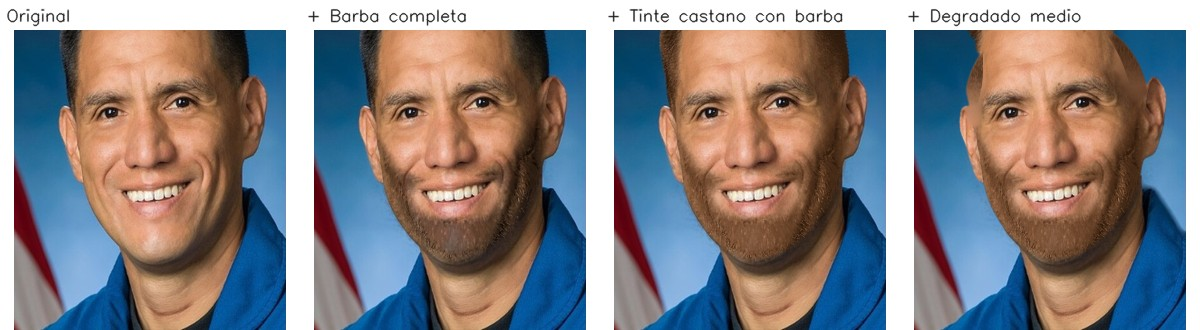
\includegraphics[width=\linewidth]{combinado.jpg}
  \caption{Look combinado sobre el retrato de ejemplo: barba completa, tinte castaño que incluye la barba y degradado medio.}
  \label{fig:combinado}
\end{figure}
